\documentclass[12pt,a4paper]{article}
\usepackage{amsmath,amssymb,mathrsfs,tikz,times,pifont}
\usepackage{enumitem}
\usepackage{float}
\newcommand\circitem[1]{%
\tikz[baseline=(char.base)]{
\node[circle,draw=gray, fill=red!55,
minimum size=1.2em,inner sep=0] (char) {#1};}}
\newcommand\boxitem[1]{%
\tikz[baseline=(char.base)]{
\node[fill=cyan,
minimum size=1.2em,inner sep=0] (char) {#1};}}
\setlist[enumerate,1]{label=\protect\circitem{\arabic*}}
\setlist[enumerate,2]{label=\protect\boxitem{\alph*}}
%%%::::::by chnini ameur :::::::%%%
\everymath{\displaystyle}
\usepackage[left=1cm,right=1cm,top=1cm,bottom=1.7cm]{geometry}
\usepackage{array,multirow}
\usepackage[most]{tcolorbox}
\usepackage{varwidth}
\tcbuselibrary{skins,hooks}
\usetikzlibrary{patterns}
%%%::::::by chnini ameur :::::::%%%
\newtcolorbox{exa}[2][]{enhanced,breakable,before skip=2mm,after skip=5mm,
colback=yellow!20!white,colframe=black!20!blue,boxrule=0.5mm,
attach boxed title to top left ={xshift=0.6cm,yshift*=1mm-\tcboxedtitleheight},
fonttitle=\bfseries,
title={#2},#1,
% varwidth boxed title*=-3cm,
boxed title style={frame code={
\path[fill=tcbcolback!30!black]
([yshift=-1mm,xshift=-1mm]frame.north west)
arc[start angle=0,end angle=180,radius=1mm]
([yshift=-1mm,xshift=1mm]frame.north east)
arc[start angle=180,end angle=0,radius=1mm];
\path[left color=tcbcolback!60!black,right color = tcbcolback!60!black,
middle color = tcbcolback!80!black]
([xshift=-2mm]frame.north west) -- ([xshift=2mm]frame.north east)
[rounded corners=1mm]-- ([xshift=1mm,yshift=-1mm]frame.north east)
-- (frame.south east) -- (frame.south west)
-- ([xshift=-1mm,yshift=-1mm]frame.north west)
[sharp corners]-- cycle;
},interior engine=empty,
},interior style={top color=yellow!5}}
%%%%%%%%%%%%%%%%%%%%%%%

\usepackage{fancyhdr}
\usepackage{eso-pic}         % Pour ajouter des éléments en arrière-plan
% Commande pour ajouter du texte en arrière-plan
\AddToShipoutPicture{
    \AtTextCenter{%
        \makebox[0pt]{\rotatebox{80}{\textcolor[gray]{0.7}{\fontsize{5cm}{5cm}\selectfont PGB}}}
    }
}
\usepackage{lastpage}
\fancyhf{}
\pagestyle{fancy}
\renewcommand{\footrulewidth}{1pt}
\renewcommand{\headrulewidth}{0pt}
\renewcommand{\footruleskip}{10pt}
\fancyfoot[R]{
\color{blue}\ding{45}\ \textbf{2025}
}
\fancyfoot[L]{
\color{blue}\ding{45}\ \textbf{Prof:M. BA}
}
\cfoot{\bf
\thepage /
\pageref{LastPage}}
% Définition de l'encadré adaptatif avec fond jaune
\newtcolorbox{resultbox}{
    colback=red!30, % Fond rouge clair
    colframe=black, % Bordure noire fine
    sharp corners, % Coins nets
    boxrule=0.5pt, % Contour léger
    boxsep=2pt, % Espacement interne
    left=5pt, right=5pt, top=2pt, bottom=2pt, % Marges internes
}
\begin{document}
\renewcommand{\arraystretch}{1.5}
\renewcommand{\arrayrulewidth}{1.2pt}
\begin{tikzpicture}[overlay,remember picture]
    \node[draw=blue,line width=1.2pt,fill=purple,text=blue,inner sep=3mm,rounded corners,pattern=dots]at ([yshift=-2.5cm]current page.north) {\begingroup\setlength{\fboxsep}{0pt}\colorbox{white}{\begin{tabular}{|*1{>{\centering \arraybackslash}p{0.28\textwidth}} |*2{>{\centering \arraybackslash}p{0.2\textwidth}|} *1{>{\centering \arraybackslash}p{0.19\textwidth}|} }
                \hline
                \multicolumn{3}{|c|}{$\diamond$$\diamond$$\diamond$\ \textbf{Lycée de Dindéfélo}\ $\diamond$$\diamond$$\diamond$ } & \textbf{A.S. : 2024/2025}                                                                     \\ \hline
                \textbf{Matière: Mathématiques}                                                                                    & \textbf{Niveau : 1}\textbf{$^{er}$S2} & \textbf{Date: 16/06/2025} & \textbf{Durée : 4 heures} \\ \hline
                \multicolumn{4}{|c|}{\parbox[c]{10cm}{\begin{center}
                                                                  \textbf{{\Large\sffamily Composition n$ ^{\circ} $ 2 Du 2$ ^\text{\bf nd} $ Semestre}}
                                                              \end{center}}}                                                                                                                               \\ \hline
            \end{tabular}}\endgroup};
\end{tikzpicture}
\vspace{3cm}

\section*{\underline{Exercice 1 :} 5 pts }

Soient \( A \) et \( B \) deux points du plan tels que \( AB = 8\, \text{cm} \).

\begin{enumerate}
    \item Construisons le barycentre \( G \) des points pondérés \( (A; 1) \) et \( (B; 3) \). \hfill \textbf{0{,}1 pt}

    \( \overrightarrow{AG} =\frac{3}{4}\overrightarrow{AB} \) et \( \overrightarrow{BG} =\frac{1}{4}\overrightarrow{BA} \)

\begin{center}
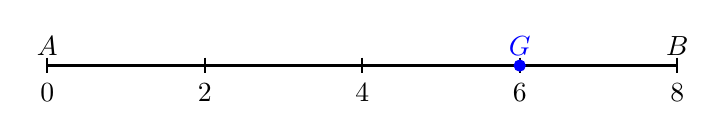
\begin{tikzpicture}
    % Segment de 8 cm
    \coordinate (A) at (0,0);
    \coordinate (B) at (8,0);

    % Tracer le segment AB
    \draw[thick] (A) -- (B);

    % Nommer les extrémités
    \node[above] at (A) {$A$};
    \node[above] at (B) {$B$};

    % Graduations à 2 cm d'intervalle
    \foreach \x in {0,2,4,6,8} {
        \draw[thick] (\x,0.1) -- (\x,-0.1);
        \node[below] at (\x, -0.1) {\x};
    }

    % Placer et nommer le point G à x=6
    \filldraw[blue] (6,0) circle (2pt) node[above] {$G$};
\end{tikzpicture}
\end{center}


    \item Calculons les distances \( GA \) et \( GB \). \hfill \textbf{0{,}5 pt + 0{,}5 pt}

\( 
        \begin{aligned}
                \overrightarrow{AG} =\frac{3}{4}\overrightarrow{AB} &\implies \| \overrightarrow{AG}\| =\frac{3}{4}\|\overrightarrow{AB}\| \\
                                                                    &\implies AG =\frac{3}{4}\times8\\
                                                                    &\implies AG =6\\
        \end{aligned} 
    \)

    \( 
        \begin{aligned}
                \overrightarrow{BG} =\frac{1}{4}\overrightarrow{BA} &\implies \| \overrightarrow{BG}\| =\frac{1}{4}\|\overrightarrow{BA}\| \\
                                                                    &\implies BG =\frac{1}{4}\times8\\
                                                                    &\implies BG =2
        \end{aligned} 
    \)
        \begin{resultbox}
            \[
                \mathbf{GA =6 \text{ et } GB =2}
            \]
		\end{resultbox}
    
    \item Démontrons que pour tout point \( M \) du plan, 
    \[
    MA^2 + 3MB^2 = 4MG^2 + 48
    \]
    \hfill \textbf{0{,}1 pt}

    \(
    \begin{aligned}
    MA^2 + 3MB^2 &= \overrightarrow{MA}^2 + 3\overrightarrow{MB}^2\\
                 &= (\overrightarrow{MG}+\overrightarrow{GA})^2 + 3(\overrightarrow{MG}+\overrightarrow{GB})^2\\
                 &= \overrightarrow{MG}^2+2\overrightarrow{MG}.\overrightarrow{GA}+\overrightarrow{GA}^2+ 3(\overrightarrow{MG}^2+2\overrightarrow{MG}.\overrightarrow{GB}+\overrightarrow{GB}^2)\\
                 &= \overrightarrow{MG}^2+2\overrightarrow{MG}.\overrightarrow{GA}+\overrightarrow{GA}^2+ 3\overrightarrow{MG}^2+6\overrightarrow{MG}.\overrightarrow{GB}+3\overrightarrow{GB}^2\\
                 &= 4\overrightarrow{MG}^2+2\overrightarrow{MG}.\overrightarrow{GA}+6\overrightarrow{MG}.\overrightarrow{GB}+3\overrightarrow{GB}^2+\overrightarrow{GA}^2\\
                 &= 4\overrightarrow{MG}^2+2\overrightarrow{MG}(\overrightarrow{GA}+3\overrightarrow{GB})+3\overrightarrow{GB}^2+\overrightarrow{GA}^2\\
                  &= 4\overrightarrow{MG}^2+2\overrightarrow{MG}(\overrightarrow{O})+3\overrightarrow{GB}^2+\overrightarrow{GA}^2\\
                  &= 4\overrightarrow{MG}^2+3\overrightarrow{GB}^2+\overrightarrow{GA}^2\\
                  &= 4\overrightarrow{MG}^2+3(2)^2+6^2\\
                  &= 4\overrightarrow{MG}^2+12+36\\
                  &= 4MG+48\\
    \end{aligned}
    \)

		        \begin{resultbox}
            \[
                \mathbf{MA^2 + 3MB^2=4MG^2+48\quad\textbf{ CQFD}}
            \]
					\end{resultbox}    
    
    \item Démontrons et construisons l'ensemble des points \( M \) du plan tels que :
    \[
    MA^2 + 3MB^2 = 84
    \]
    \hfill \textbf{0{,}1 pt}

	D'après la relation précédente on a \( MA^2 + 3MB^2=4MG^2+48 \)

		    \(
    \begin{aligned}
    		4MG^2+48 &= 84\\
        4MG^2 &= 84-48\\  
         4MG^2 &=36\\
         MG^2 &=9\\
         MG &=3\\
    \end{aligned}
    \)    
    
    Donc, l'ensemble des points \( M \) tels que \( MA^2 + 3MB^2 = 84 \) est le cercle de centre \( I \) et de rayon \( 3 \) :   
    		    \begin{resultbox}
            \[
                \mathbf{\mathscr{C}(I,\;3) }
            \]
					\end{resultbox} 
    
    \item Déterminons et construison l'ensemble des points \( M \) tels que :
    \[
    \overleftarrow{MA}\cdot\overleftarrow{MB} = -12
    \]
    \hfill \textbf{0{,}1 pt}

		Soit \(I\) milieu de \(AB\)  
		
		\(		
		\begin{aligned}
			\overrightarrow{MA} \cdot \overrightarrow{MB} = -12 &\implies \overrightarrow{MI}^{2}-\frac{\overrightarrow{AB}^{2}}{4} = -12\\
			&\implies \overrightarrow{MI}^{2}-\frac{8^{2}}{4} = -12\\
			&\implies \overrightarrow{MI}^{2}-16 = -12\\
			&\implies \overrightarrow{MI}^{2} = 4\\
		\end{aligned}
		\)  

Donc, l'ensemble des points \( M \) tels que \( \overrightarrow{MA} \cdot \overrightarrow{MB} = -12 \) est le cercle de centre \( I \) et de rayon \( 2 \) :   
    		    \begin{resultbox}
            \[
                \mathbf{\mathscr{C}(I,\;2) }
            \]
					\end{resultbox}  
\end{enumerate}

\end{document}